\chapter{Research Context}
\graphicspath{{Chapter2/Figs/}{Chapter2/Figs/}}

This chapter describes the research question's context and the current literature findings. The reader is educated on the limitations of current non-invasive and unidirectional BCIs, the paradigm shift in developing cloud-based and production-ready software versus running software in a research environment, and the implications and hypotheses of web-based approaches to BCIs and 3D applications for VR and AR that relate to the future of software in general in the field of spatial computing.

\section{Limitations of BCIs}
\label{chapter2-limitations-of-bcis}

The capabilities of BCIs are not without limitations. In addition to the physical limitations, mainly in material science for the hardware aspects of BCIs, the author attempts to address a broader issue related to neuropsychology that directly correlates to the software aspects.

\subsection{Decoding brain data}
\label{chapter2-decoding-brain-data}

As outlined in the previous chapter, a holistic view of BCI must take into account the aspect of decoding measured neural data and making it intelligible to computer software. It is important to emphasise that the task of decoding neural data is different from decoding thoughts, which is a critical factor for software. Moreover, decoding neural data and extracting the thoughts behind it so that the software can understand them are disciplines on their own. For example, getting computers to recognise letters written on a photograph is a very different problem from reading the written words in the sentences (i.e. computer vision and natural language processing).

Another part is understanding the sentences and their meaning, as in natural language understanding (NLU). NLU is considered an AI-hard problem, which means that the difficulty of these computational problems is equivalent to solving the central problem of artificial general intelligence (AGI) \citep{demasi_theoretical_2010}, assuming that general human-level intelligence is computational. Understanding less structured data, such as EEG data, is more complicated than understanding structured and human-generated syntax such as written language because it contains more hidden features than a paragraph of text. As a result, the author assumes that understanding brain data might be considered an AI-hard problem.

\subsection{Abstract thoughts}
\label{chapter2-abstract-thoughts}

\begin{figure}[ht]
  \centering
  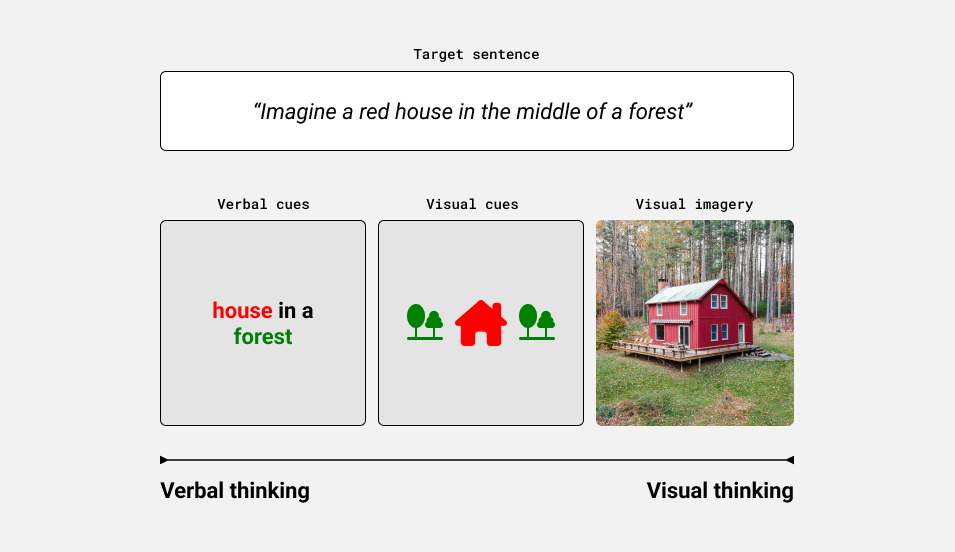
\includegraphics[width=\linewidth]{visual-thinking.png}
  \caption{Difference between verbal and visual thinking using the target sentence of a red house in the middle of a forest (own representation, 2022).}
  \label{fig:visual-thinking}
\end{figure}

Imagine a red house in the middle of a forest. Depending on the individual thought process, one can imagine the house with temporary visual imagery in mind, as in visual thinking, or one can imagine it more verbally, such as conceptually comprehending each word sequentially of what a red house is and that it is located in a forest \citep{amit_asymmetrical_2017}. Additionally, it should also be addressed that different types of thoughts exist at different levels of abstraction and complexity. One can assume that the visual image of a red house in the forest is more abstract and far-fetched than, say, the movement of one's own thumbs, which has a clear physical counterpart. It gets even more complicated when one imagines concepts that are inconceivable to visualise, such as the idea of a company. A company is only an abstract, collectively agreed upon concept without a physical counterpart and is, therefore, even less straightforward and more complex to decode the meaning of measured brain activity than the other mentioned examples of the red house.

\subsection{Technological limitations}
\label{chapter2-technological-limitations}

\begin{figure}[ht]
  \centering
  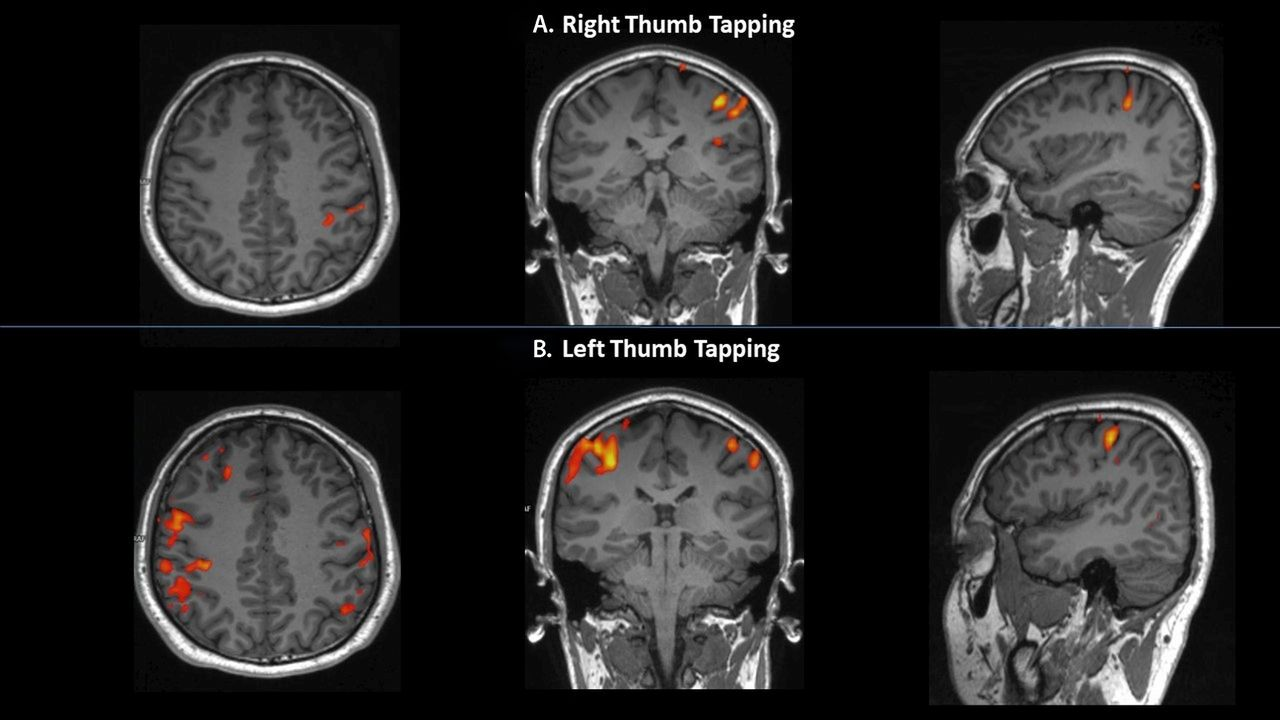
\includegraphics[width=\linewidth]{fmri-scan.jpg}
  \caption{Image of localised activation of neurons during right and left thumb movement using functional magnetic resonance imaging (fMRI) \citep{rashid_bilateral_2018}.}
  \label{fig:fmri-scan}
\end{figure}

Functional tasks of the brain are localised, which means that these signals are generated by local brain areas that can be identified, such as the motor cortex, which has been shown to be responsible for muscle movement as shown in Figure \ref{fig:fmri-scan}. Examining the areas of the brain responsible for activating individual muscle strands can yield a comparable response of muscle stimulation in the brain and thus be measured as output for software to move a prosthesis, for example. However, the more specific, less functional, more behavioural and abstract the thoughts are, the less the brain areas are spatially visible. The intent of identifying, for example, the thought of a red house in a forest in verbal thought, the author identified three technological problem statements:

\begin{itemize}
  \item To understand single thoughts, it is essential to have sufficiently clear data from experiments with a certain level of detail (e.g., at the level of detail related to the firing of action potential of individual neurons) as well as temporal precision (an action potential takes about 1 ms to arise) to perform studies to extract possible localisations of individual thoughts. Current neuroimaging technologies cannot capture every process in sufficient detail of the entire brain at once to extract the activity of, e.g. individual neurons while also having high temporal precision.
  \item Even if we could measure every single neuron in the brain with high temporal precision, we would have an extreme amount of data generated concisely. Let us say we would collect a float per neuron that represents the rate of change in voltage with respect to time in milliseconds and then record each neuron in the brain a million times a second, taking into account that the average human brain has around 86 billion neurons; we would generate 305.53337637684 petabytes of data per second. This is currently not feasible for most of the commercially available storage and processing resources available.
  \item Even if we have the technology, it is a challenge because reproducibility of experiments is very difficult for neuroscientific studies. It is probably impossible to generate clean-slate neural data that is comparable to previously recorded data. Our neurophysiological brain structure changes over time due to neuroplasticity \citep{puderbaugh_neuroplasticity_2022}, and we are in different states of mind every millisecond of our existence, which can have different influences, such as insufficient sleep, something disturbing someone, mental distraction due to an important event that may have occurred since the last measurement, or a salient thought that occurs during a measurement.
\end{itemize}

\subsection{Lack of data}
\label{chapter2-lack-of-data}

As pointed out in the previous section, points 2 and 3 depend on advances in data storage systems or the possibility that we do not actually need 3such precise brain data to understand single thoughts. However, to address point 1, some promising solutions already exist for measuring large parts of the brain with high temporal and spatial precision, such as time-domain functional near-infrared spectroscopy (TD-fNIRS), which Kernel employs in its Kernel Flow device. The TD-fNIRS system detects changes concentrations of oxygenated (oxyHb) and deoxygenated brain cell activity by using near-infrared light in response to neuronal activity. This is a newer and more promising technology for measuring the full spectrum of neuroimaging of brain activity when compared to EEG. According to Kernel's, the precision of TD-fNIRS is sufficient for better understanding the brain and using it for BCI applications. They, however, claim that collecting and organising longitudinal brain data from a variety of subjects is the key to solving the most difficult challenges in neuroscience \citep{kernel_hello-humanitypdf_nodate}.

Based on Kernel's claim, a recent publication from 2022 also claims that even data sets with several hundred people are too tiny to consistently offer insights about the brain \citep{marek_reproducible_2022}. As a result, most published brain-wide association studies with dozens or even hundreds of people could all be incorrect. In such research, variations in brain structure and activity have been linked to variances in cognitive capacity, mental health, and other behavioural features. Numerous studies, for example, have revealed brain structure or activity patterns that may help distinguish persons with depression from those who are not. Neuromarkers of behavioural features is frequently sought in studies. The recent publication from \citeauthor{marek_reproducible_2022} claims that most of these so-called neuro markers would not work when the collected data set is more extensive, which prose a general problem for the field of neuroscience.

This is both fascinating and a significant constraint for BCIs, because understanding the brain is essential to making sense of the measured and classified data for interfacing with it. Therefore a large amount of brain data collected in reproducible experiments is a must for production-ready and mainstream-ready BCIs. UK Biobank's collection of brain scans is one of the first efforts to solve this problem \citep{noauthor_imaging_nodate}, but it is still far from what we might need. Marek himself claims that we might even need millions of data sets to start understanding the brain \citep{callaway_can_2022}.

\section{BCI landscape}
\label{chapter2-research-landscape}

% Summarise based on limitations the current products, their sample rates, spatial resolution, form factors and software offerings
% Current landscape of non-invasive BCIs and their applications (take IDUN's competition overview as a starter point)

\subsection{Real-world BCI applications}
\label{chapter2-real-world-bci-applications}

% Current state of EEG-based games and applications for the normal user (steady state invoked etc.) (talk with Michel and do own research)

% everything is a neural interface, even our own body

% external stimuli, like a sound or light

% personal thoughts: active and passive; make difference of wearable and passive

% "sinnesorgan": motor stuff, visual, auditory, neurofeedback (learn how to control your thoughts, attention training for adhs e.g.) etc.

\subsection{Unobtrusive hardware and software}
\label{chapter2-unobtrusive-hardware-and-software}

% What it takes for a BCI to be mainstream-ready with IDUN as an example (talk with Simon and example of smart glasses)

\subsection{Active and passive BCIs}
\label{chapter2-active-and-passive-bcis}

% Passive brain-computer interfaces and user experience (read paper on passive brain-computer interfaces)

\section{Production-grade software}
\label{chapter2-production-grade-software}

% What production-grade software separates from others
% Use The Twelve Factors as a reference

\subsection{Cloud paradigm-shift}
\label{chapter2-cloud-paradigm-shift}

% Challenges and requirements of going with a cloud, API and SDK (privacy, security, IP, performance, scaling etc.)

\subsection{Web-first BCI architecture}
\label{chapter2-web-first-bci-architecture}

% Examples of BCI data going through web stacks, how to make it work (paper from Stegman)

\subsection{3D applications in the browser}
\label{chapter2-3d-applications-in-the-browser}

% Current state of 3D on the web (WebGPU, pixel streaming, declarative graphics components, WebAssembly (and Rust), etc.)

\subsection{Web-based AR and VR}
\label{chapter2-web-based-ar-and-vr}

% Current state of VR and AR applications (Meta Quest, Snapchat, ARKit, etc.)

\section{N/CI challenges}
\label{chapter2-nci-challenges}

% General challenges of a N/CI

% Akademischer Hintergrund: Vorbilder, Referenzmaterial, Eingrenzung und vertiefte Begründung der Zielformulierung. Grundlagenforschung im Bereich vergleichbarer Medienprodukte. Kenntnis der fachspezifischen Theorien und Techniken. Hier muss umfassende Fach- und Handwerkskenntnis gezeigt werden. Es sollen möglichst viele Informationen verwendet werden, die helfen sollen Entscheidungen für die Erstellung des eigenen Medienprodukts zu treffen und Vorgehensweisen beim Entstehungsprozess des eigenen Medienprodukts zu begründen. Ebenso soll begründet werden, inwiefern die verwendeten Quellen für die Zielsetzung und deren Umsetzung geeignet sind.

\nomenclature[nlu]{NLU}{Natural language understanding}
\nomenclature[agi]{AGI}{Artificial general intelligence}
\nomenclature[fmri]{fMRI}{Functional magnetic resonance imaging}
\nomenclature[tdfnirs]{TD-fNIRS}{Time-domain functional near-infrared spectroscopy}
